%% ****** Start of file apstemplate.tex ****** %
%%
%%
%%   This file is part of the APS files in the REVTeX 4.2 distribution.
%%   Version 4.2a of REVTeX, January, 2015
%%
%%
%%   Copyright (c) 2015 The American Physical Society.
%%
%%   See the REVTeX 4 README file for restrictions and more information.
%%
%
% This is a template for producing manuscripts for use with REVTEX 4.2
% Copy this file to another name and then work on that file.
% That way, you always have this original template file to use.
%
% Group addresses by affiliation; use superscriptaddress for long
% author lists, or if there are many overlapping affiliations.
% For Phys. Rev. appearance, change preprint to twocolumn.
% Choose pra, prb, prc, prd, pre, prl, prstab, prstper, or rmp for journal
%  Add 'draft' option to mark overfull boxes with black boxes
%  Add 'showkeys' option to make keywords appear
%\documentclass[aps,prl,preprint,groupedaddress]{revtex4-2}
\documentclass[aps,twocolumn,groupedaddress]{revtex4-2}
%\documentclass[aps,prl,preprint,superscriptaddress]{revtex4-2}
%\documentclass[aps,prl,reprint,groupedaddress]{revtex4-2}

% You should use BibTeX and apsrev.bst for references
% Choosing a journal automatically selects the correct APS
% BibTeX style file (bst file), so only uncomment the line
% below if necessary.
%\bibliographystyle{apsrev4-2}

\usepackage{graphicx}
\usepackage{epstopdf}
%\usepackage{amsmath}% http://ctan.org/pkg/amsmath
%\usepackage{amsthm}
%\usepackage{amsfonts}
%\usepackage{subfigure}
%\usepackage{hhline}
%\usepackage[miktex]{gnuplottex}
%\usepackage{xcolor}
\usepackage{amssymb}
\usepackage{amsmath}
\usepackage{color}
\usepackage{comment}
\usepackage{hyperref}
%\usepackage[percent]{overpic}
\usepackage{tikz}
\usepackage{mathrsfs}
\usepackage{wasysym}
\usepackage{tikz-cd}
%\usepackage{stix} %\fisheye
\usepackage{stackengine,scalerel}
\usepackage{float}
\usepackage{multirow}
\usepackage{booktabs}
\usepackage{subcaption}
\usepackage[spanish]{babel}
\usepackage{titlesec}


% so sections, subsections, etc. become numerated.
\setcounter{secnumdepth}{3}

% Comandos proprios
\DeclareMathOperator*{\argmax}{arg\,max}
\DeclareMathOperator*{\argmin}{arg\,min}
\newcommand{\avrg}[1]{\left\langle #1 \right\rangle}
\newcommand{\nelta}{\bar{\delta}}
\newcommand{\bra}[1]{\left\langle #1\right|}
\newcommand{\ket}[1]{\left| #1 \right\rangle}
\newcommand{\sbra}[1]{\langle #1|}
\newcommand{\sket}[1]{| #1 \rangle}
\newcommand{\bek}[3]{\left\langle #1 \right| #2 \left| #3 \right\rangle}
\newcommand{\sbek}[3]{\langle #1 | #2 | #3 \rangle}
\newcommand{\braket}[2]{\left\langle #1 \middle| #2 \right\rangle}
\newcommand{\ketbra}[2]{\left| #1 \middle\rangle \middle\langle #2  \right|}
\newcommand{\sbraket}[2]{\langle #1 | #2 \rangle}
\newcommand{\sketbra}[2]{| #1 \rangle  \langle #2 |}
\newcommand{\norm}[1]{\left\lVert#1\right\rVert}
\newcommand{\snorm}[1]{\lVert#1\rVert}
\newcommand{\bvec}[1]{\boldsymbol{\mathsf{#1}}}
\newcommand{\bcov}[1]{\boldsymbol{#1}}
\newcommand{\bdua}[1]{\boldsymbol{\check{#1}}}
%\newcommand{\bdov}[1]{\boldsymbol{\breve{#1}}}
\newcommand{\bdov}[1]{\breve{#1}}
%\newcommand{\bten}[1]{\boldsymbol{\mathfrak{#1}}}
\newcommand{\bten}[1]{\boldsymbol{\mathfrak{#1}}}
\newcommand{\forany}{\tilde{\forall}}
\newcommand{\qed}{$\overset{\circ}{.}\;$}

\newcommand\bigeye{\ensurestackMath{\stackinset{c}{}{c}{-.3pt}%
  {\bullet}{\scriptstyle\bigcirc}}}
\newcommand\eye{\scalerel*{\bigeye}{x}}
%\newcommand*{\fisheye}{%
%    \mathbin{%
%        \ooalign{$\circledcirc$\cr\hidewidth$\bullet$\hidewidth}%
%    }%
%}
\renewcommand{\appendixname}{Apéndice} % Change "Appendix" to "Apéndice"

\begin{document}

% Use the \preprint command to place your local institutional report
% number in the upper righthand corner of the title page in preprint mode.
% Multiple \preprint commands are allowed.
% Use the 'preprintnumbers' class option to override journal defaults
% to display numbers if necessary
%\preprint{}

%Title of paper
\title{
Primeros Pasos en Redes Neuronales: Clasificando Fashion-MNIST con PyTorch
}

% repeat the \author .. \affiliation  etc. as needed
% \email, \thanks, \homepage, \altaffiliation all apply to the current
% author. Explanatory text should go in the []'s, actual e-mail
% address or url should go in the {}'s for \email and \homepage.
% Please use the appropriate macro foreach each type of information

% \affiliation command applies to all authors since the last
% \affiliation command. The \affiliation command should follow the
% other information
% \affiliation can be followed by \email, \homepage, \thanks as well.
\author{Benjamín Bas Peralta}
\email[]{benjamin.bas@mi.unc.edu.ar}
%\homepage[]{Your web page}
%\thanks{}
%\altaffiliation{}
%\affiliation{}
\affiliation{Facultad de Matem\'atica, Astronom\'ia, F\'isica y Computaci\'on, Universidad Nacional de C\'ordoba, Ciudad Universitaria, 5000 C\'ordoba, Argentina}

%Collaboration name if desired (requires use of superscriptaddress
%option in \documentclass). \noaffiliation is required (may also be
%used with the \author command).
%\collaboration can be followed by \email, \homepage, \thanks as well.
%\collaboration{Juan Perez}
%\noaffiliation
\date{22 de Noviembre de 2024}

\begin{abstract}
El Aprendizaje Automático (del inglés \textit{Machine Learning}, ML) es el campo dentro de Ciencias de la Computación cuyo objetivo es desarrollar técnicas que permitan que las computadoras \textit{aprendan} a partir de la \textit{experiencia}, sin la necesidad de ser explícitamente programadas para hacerlo. Una de estas técnicas, y que es la que en los últimos años ha tenido el mayor crecimiento gracias a su capacidad de aplicación en una infinitud de áreas, es la de Redes Neuronales Artificiales, cuya inspiración está en la arquitectura del cerebro animal. En este informe, daremos los conceptos básicos acerca de su funcionamiento, y veremos cómo nos ayudarán a resolver un problema de clasificación sobre imágenes de prendas de ropa utilizando una librería de Python llamada PyTorch.
\end{abstract}

% insert suggested keywords - APS authors don't need to do this
%\keywords{}

%\maketitle must follow title, authors, abstract, and keywords
\maketitle

\section{Introducción}
Los algoritmos de Aprendizaje Automático, también llamados \textbf{modelos}, son capaces de \textbf{aprender} a partir de los datos. Pero, ¿a qué nos referimos con ``aprender''? En 1997, Tom Mitchell lo definió de la siguiente manera: ``Se dice que un programa de computadora aprende de la experiencia E con respecto a una clase de tareas T y una medida de desempeño P, si su desempeño en las tareas de T, medido por P, mejora con la experiencia E''. Con esta definición en mente, si bien existen numerosas tareas que pueden ser resueltas con ML, dos de las más comunes son regresión, que consiste en predecir un valor continuo, y clasificación, que consiste en predecir un valor categórico y será en la que nos enfocaremos en este informe. 

Con respecto a la experiencia, estos algoritmos se pueden clasificar en supervisados y no supervisados, haciendo alusión a la información que ``pueden ver'' durante su proceso de aprendizaje \cite{hands-on-ML-sklearn-tf}, muy comúnmente llamado proceso de \textit{entrenamiento}. El caso estudiado en este informe forma parte de los primeros, en donde el algoritmo aprende a partir de un conjunto de datos - \textit{dataset} - compuesto por entradas y el valor esperado (la ``etiqueta'') para cada una de ellas. A este subconjunto del dataset se lo suele conocer como ``conjunto de entrenamiento''.

Por último, para medir el desempeño en estos algoritmos, se definen métricas cuantitativas que dependen de la tarea que se esté realizando. Por ejemplo, en clasificación, una de las más comunes es la de exactitud - \textit{accuracy} -, que es la proporción de ejemplos para los cuales el modelo predijo la salida correcta (dada por el dataset). El objetivo fundamental del ML es generalizar más allá de los ejemplos del conjunto de entrenamiento \cite{pedro-domingos}. Por lo tanto, para evaluar qué tan bien se comporta el modelo, su rendimiento se mide en un subconjunto del dataset distinto con el que aprendió, llamado ``conjunto de test''.

En este ensayo, hablaremos sobre las Redes Neuronales Artificiales (RNA), un algoritmo particular dentro del ML, y experimentaremos con ellas sobre un problema de clasificación de imágenes de prendas de ropa utilizando el dataset Fashion-MNIST (\cite{fashion-mnist}), del cual hablaremos más adelante.  Para llevar a cabo los experimentos, utilizaremos la librería de diferenciación automática PyTorch (\cite{pytorch}) del lenguaje de programación Python, la cual facilita en gran medida el entrenamiento de Redes Neuronales.

\textit{Organización del artículo.} En la sección 2, hablaremos sobre el funcionamiento teórico de las RNAs y cómo se entrenan, explicando los conceptos fundamentales necesarios para comprender lo que haremos durante la experimentación. Luego, en la sección 3, mostraremos los resultados obtenidos en los distintos experimentos variando ciertos ajustes del modelo. En la sección 4, haremos un enfoque más cuantitativo sobre lo obtenido para dar una conclusión. Finalmente, realizamos un resumen con los aportes más importantes del trabajo.

\section{Teor\'ia}
Las RNAs son un modelo específico dentro del Aprendizaje Automático, cuya estructura y funcionamiento están inspirados en los del cerebro. Durante los últimos años, ha sido el área que más desarrollo e impacto ha tenido, principalmente gracias a su versatilidad, potencia y escalabilidad, cualidades que hacen que sean capaces de enfrentar problemas grandes y complejos \cite{hands-on-ML-sklearn-tf}. Entre algunos de estos, se encuentran el reconocimiento facial y de voz, sistemas de recomendación, y la clasificación de imágenes, que es el objetivo de nuestro trabajo. 

\begin{comment}
\subsection{Breve Contexto Histórico}
Aunque su gran éxito ha sido reciente, lo cierto es que la idea de las RNAs data desde 1943, cuando Warren McCulloch y Walter Pitts presentaron en su artículo ``A Logical Caclulus of Ideas Immanent of Nervous Activity'' un modelo computacional simplificado utilizando lógica proposicional acerca de cómo funcionan las neuronas de cerebros animales en conjunto para llevar a cabo cómputos complejos \cite{hands-on-ML-sklearn-tf}. 

Posteriormente, en 1957, Frank Rosenblatt presentó una de las arquitecturas más simples de RNAs: el ``Perceptrón'', el cual sirve principalmente para resolver problemas de clasificación en donde los datos son linealmente separables. Su aporte más notorio es que definió un algoritmo para su entrenamiento, el cual estaba basado fuertemente en la regla de Hebb, presentada en 1949, que establece a grandes rasgos que el secreto de la inteligencia artificial no está en la complejidad de las neuronas, sino en la complejidad de la arquitectura de conexiones entre neuronas, llamadas sinapsis \cite{apuntes-redes-neuronales}.

Más tarde, se descubrió que los problemas que no podían ser resueltos por el Perceptrón, sí podían ser resueltos ``apilando'' múltiples perceptrones, lo cual llevó a la invención del ``Perceptrón Multicapa'' (PMC), también conocido como ``Redes Neuronales de Propagación Directa'' (del inglés \textit{Feedforward Neural Networks}) \cite{deep-learning}. Si bien hasta el día de hoy se han creado diferentes arquitecturas pensadas para problemas específicos, en este ensayo nos abocaremos a estudiar la arquitectura \textit{feedfoward}.
\end{comment}

\subsection{Elementos de una Red Neuronal}
El elemento básico de cualquier red neuronal es la \textbf{neurona}, que es la que lleva a cabo el ``cómputo''. Una neurona está conectada con otras, de las cuales recibe información y a quienes también les envía. Estas conexiones representan las \textbf{sinapsis} y cada una tiene asociada un determinado número llamado \textbf{peso}, que simboliza la intensidad de la conexión. De esta manera, el trabajo que lleva a cabo una neurona es primero computar una suma pesada de sus entradas: \( z = w_1x_1 + w_2x_2 + … + w_nx_n = w^T x\), donde \(x_i\) representa la entrada proveniente de la neurona \(i\) y \(w_i\) es el peso asociado a esta conexión. Y sobre este valor resultante, aplica una \textbf{función de activación} \(h\), siendo como resultado final de la neurona \(h(z) = h(w^T x)\). Esto se puede ver gráficamente en la figura \ref{fig:neuron}.

\begin{figure}[h!]
    \centering
    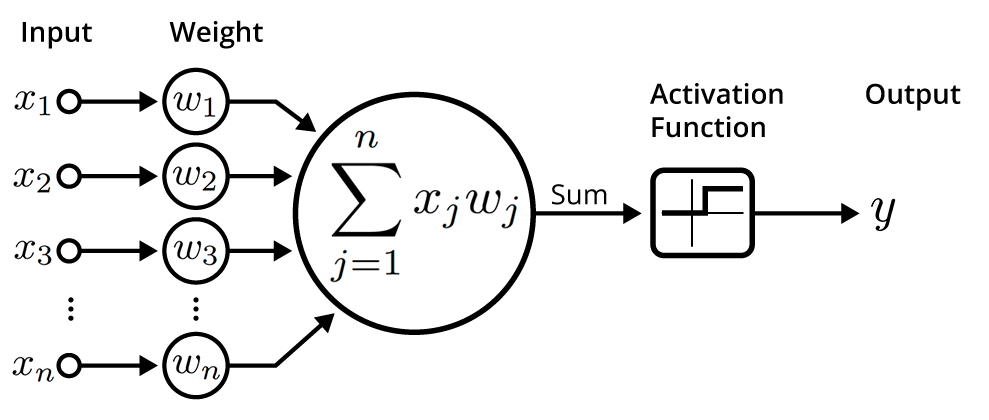
\includegraphics[width=0.35\textwidth]{figs/neuron.png}
    \caption{La neurona computa una suma pesada de sus entradas y aplica una función de activación sobre el resultado.}
    \label{fig:neuron}
\end{figure}

La idea detrás de la función de activación es el hecho de propagar la información proporcionalmente al estímulo provocado por las entradas en la neurona, basándose en la idea de ``disparo'' de una neurona biológica en el momento en que se supera el umbral de activación. La función de activación utilizada en el Perceptrón, uno de los primeros modelos de RNAs, fue la llamada \textit{heavyside}, dada por \(\text{heavyside}(z)=0\text{ si }z < 0; 1\text{ si } z\geq0\). 

Durante los años, se han empleado diferentes funciones de activación, como la sigmoide, la tangente hiperbólica, y la ReLU, dada por \(\text{ReLU}(z)=\text{max}(0, z)\), siendo esta última la más común actualmente.

Dicho esto, una red neuronal está compuesta por diferentes capas de neuronas: la capa de entrada, que es por donde ingresan los datos, una o más capas ocultas o intermedias, en donde aparecen las funciones de activación, y finalmente la capa de salida. En una red \textit{feedforward} particularmente, las neuronas de una capa están conectadas solamente con las neuronas de la capa siguiente, implicando de esta forma que la información fluye solamente en una dirección (de aquí la nomenclatura \textit{feedforward}). Algo a notar también sobre estas redes es que todas las capas están totalmente conectadas entre sí, como puede verse en la figura \ref{fig:neural-net}.

\begin{figure}[h!]
    \centering
    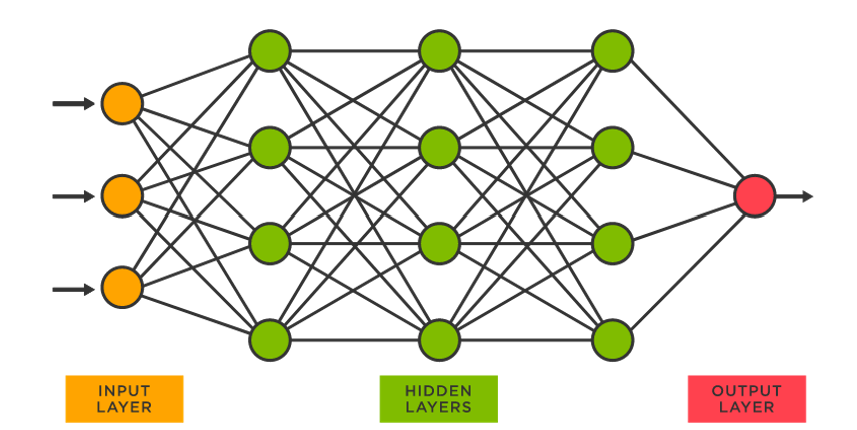
\includegraphics[width=0.35\textwidth]{figs/feedforward.png}
    \caption{Esquema de una Red Neuronal Profunda, con tres capas ocultas. Las neuronas naranjas forman la capa de entrada, las neuronas verdes forman las tres capas ocultas, y las rojas la de salida.}
    \label{fig:neural-net}
\end{figure}

Ahora bien, el objetivo de una red neuronal es \textbf{aproximar una función desconocida} \(g^*\). Para un clasificador por ejemplo, \(y=g^*(x)\) determina una categoría \(y\) para una entrada \(x\). De esta forma, una red define una asignación \(y=g(x; \theta)\) y aprende el valor de los \textbf{parámetros} \(\theta\) que resultan en la mejor aproximación de la función ``oculta'' \cite{deep-learning}. En este caso, los parámetros a aprender por la red serán los pesos sinápticos de todas las conexiones. Matemáticamente, los pesos entre una capa de neuronas y la siguiente se pueden pensar como una matriz \(w\), en donde la entrada \(w_{ij}\) indica el peso sináptico de la conexión entre la neurona \(i\) de la capa ``actual'' y la neurona \(j\) de la capa ``anterior''. La pregunta que surge entonces es \textbf{cómo} hacer para que la red pueda aproximar esta función.

\subsection{Entrenamiento de una Red Neuronal Feedforward}
A grandes rasgos, el entrenamiento de una red consiste en una suma de \textbf{evaluación} y \textbf{optimización} \cite{pedro-domingos}. Con evaluación, nos referimos al establecimiento de una medida que determine qué tan lejos está el modelo de hallar una buena solución, para lo cual se suele definir una función a minimizar o maximizar llamada \textbf{función objetivo} o \textbf{criterio} \cite{deep-learning}; y la optimización es el método usado para aproximarse a dicha solución, maximizando o minimizando la función objetivo según corresponda.

Cuando lo deseado es minimizar la función objetivo, esta pasa a ser llamada \textbf{función de costo}, \textbf{función de error} o \textbf{función de pérdida}. En problemas de aprendizaje supervisado, esta función compara la salida de la red para determinadas entradas - la predicción - en el estado actual de la red, dado por el valor de los pesos sinápticos en ese momento, con las salidas reales para dichas entradas, dadas por el conjunto de entrenamiento. En resumen, una vez que están fijos los datos del conjunto de entrenamiento, la función de costo es una función de los pesos de la red. Por lo tanto, la denotaremos con \(f(w)\).

Dos de las funciones de costo más utilizadas son el Error Cuadrático Medio y la \textbf{Entropía Cruzada}. De estas dos funciones, nos concentraremos en la última ya que es la más apropiada para problemas de clasificación como el que tratamos. Esto se debe a que mide la diferencia entre la distribución de probabilidad predicha por el modelo y la distribución real de los datos.  En este caso, la capa de salida tiene tantas neuronas como categorías haya, y la salida de cada una de ellas representa el puntaje que le da la red a la categoría correspondiente a cada neurona, donde un mayor puntaje indica una mayor probabilidad de pertenencia de la entrada particular a dicha clase. Para obtener una estimación de la distribución de probabilidad dada por estas salidas, se aplica la función \textit{softmax} \cite{hands-on-ML-sklearn-tf}.

Una vez que se tiene esta función establecida y se calculan las pérdidas para los datos, el algoritmo por defecto que se utiliza para la optimización es el de \textbf{Descenso por el Gradiente} (\textit{Gradient Descent}). Este se basa en modificar los parámetros (i.e. los pesos sinápticos) iterativamente con el objetivo de encontrar mínimos locales de una función, que en este caso será la de costo. Se basa en la idea que la dirección dada por el gradiente es la de mayor crecimiento, y por lo tanto su opuesta es la de menor. De esta forma, lo que se hace en cada paso es calcular el gradiente de la función de costo con respecto a los pesos, y luego actualizarlos siguiendo la siguiente regla:
\[
w = w - \eta \ \nabla f(w),
\]
donde \(w\) representa una matriz de pesos de una determinada capa, y la cantidad \(\eta\) es llamada la \textbf{tasa de aprendizaje}, que determina el tamaño de cada paso. Si \(\eta\) es muy pequeño, entonces el algoritmo tendrá que hacer muchos pasos para converger; pero si es demasiado grande, puede llegar a divergir. 

Actualmente, se utilizan otros optimizadores más sofisticados y eficientes, pero que todos parten de la idea del Descenso por el Gradiente. Los que usaremos en los experimentos son el Descenso por el Gradiente Estocástico (\textit{Stochastic Gradient Descent}, SGD) y Adam (\textit{Adaptive Moment Estimation}), de los cuales se puede leer más en el Capítulo 8 de \cite{deep-learning}.

Ahora bien, recordando que la función \(f\) está fija en todas las entradas y salidas del conjunto de entrenamiento, hay algoritmos de optimización que utilizan todos estos datos para  calcular el gradiente, otros que utilizan de a un ejemplo a la vez para calcular el gradiente y otros que están entre medio de los dos anteriores, es decir utilizan un subconjunto del conjunto de datos para calcular el gradiente (esto es lo que hace SGD). 

Es necesario en este punto introducir el concepto de ``\textbf{época}'' y de ``\textbf{lote}''. Un lote es simplemente una subdivisión de tamaño fijo del conjunto de entrenamiento (o de test). Dicho esto, se llama época al proceso completo en el cual el modelo entrena utilizando \textbf{todos} los datos disponibles en el conjunto de entrenamiento una vez, ya sea recorriéndolos de a lotes o todos de una vez. Si el conjunto está efectivamente dividido en lotes, una época va a consistir de: \textbf{para cada lote}, calcular las predicciones en base a los pesos actuales, obtener los errores de cada muestra del lote, computar los gradientes en base a los ejemplos del lote y actualizar los pesos. Si no, se hacen los mismos pasos pero para todos los datos de una vez.

Al entrenar un modelo, existen ciertos ajustes que son utilizados para controlar su comportamiento llamados \textbf{hiperparámetros}. Los valores de los hiperparámetros no son aprendidos por el modelo \cite{deep-learning}, sino que se fijan de antemano y no se modifican a lo largo del entrenamiento. Algunos de estos son: la cantidad de neuronas en cada capa oculta, la función de activación utilizada en cada capa, el optimizador, la tasa de aprendizaje, el número de épocas, el tamaño de lote, entre otros. Todos estos pueden contribuir a que el modelo mejore su desempeño. Para probar distintos valores de hiperparámetros, que es lo que haremos a continuación, se utiliza un conjunto de datos extra además del de entrenamiento y el de test, llamado de \textbf{validación} que sirve justamente para encontrar los hiperparámetros óptimos.

Otras mejoras que se han implementado para mejorar la eficacia de los modelos, y que emplearemos en los experimentos, son las nombradas a continuación. Por un lado, tenemos la \textbf{detención temprana}, que consiste en frenar el entrenamiento en el último mejor ``estado'' del modelo cuando se observa que a partir de dicho punto el error sobre el conjunto de validación no mejora (notar que cuántas épocas se espera y qué se considera una mejora son nuevos hiperparámetros). Y por otro lado, el \textbf{dropout}, que es un algoritmo que implica suprimir un cierto número de neuronas de una capa de manera aleatoria \cite{apuntes-redes-neuronales}. 

\section{Resultados}
Como mencionamos en la Introducción, la tarea que intentaremos resolver aquí utilizando Redes Neuronales es la de clasificación de imágenes de diferentes prendas de ropa, haciendo uso del dataset Fashion-MNIST. Partiremos de una arquitectura base con determinados hiperparámetros y a lo largo de los diferentes experimentos iremos modificándolos, por lo que tendremos un conjunto de entrenamiento y un conjunto de validación (no hay conjunto de test).

Fashion-MNIST es un conjunto de datos que fue creado en 2017 y está compuesto por 70000 imágenes en escala de grises de 28 por 28 píxeles de 10 categorías de prendas de ropa distintas, habiendo 7000 imágenes por categoría.  El conjunto de entrenamiento tiene 60000 imágenes y el de test 10000 \cite{fashion-mnist}. Ejemplos de estas imágenes, junto con la clase a la que pertenecen, se pueden ver en la figura \ref{fig:fashion-mnist-samples}.

\begin{figure}[h!]
    \centering
    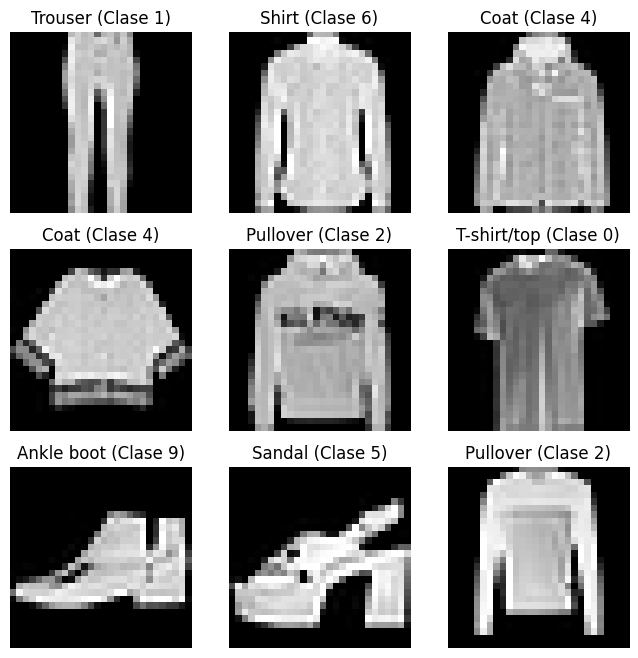
\includegraphics[width=0.25\textwidth]{figs/fashion-mnist-samples.png}
    \caption{Muestras de las imágenes presentes en el dataset Fashion-MNIST junto con su clase.}
    \label{fig:fashion-mnist-samples}
\end{figure}

Las métricas en las que nos concentraremos para medir el desempeño del modelo serán la \textbf{exactitud} sobre cada conjunto, y el \textbf{error promedio por lote}, esto es el valor promedio devuelto por la función de pérdida a lo largo de todos los lotes de una época. 

Cabe aclarar que en todos los experimentos el número \textit{máximo} de épocas de entrenamiento usado fue 100, con la técnica de detención temprana, poniendo como criterio de parada que no hubo una disminución de al menos 0.0001 en la pérdida del conjunto de validación por 20 épocas seguidas. Esto provoca que no en todos los experimentos la cantidad de épocas totales de entrenamiento sea la misma. Dicho esto, la última época mostrada en los gráficos  a continuación es a partir de la cual se cuentan las 20 de no mejoría.

En esta sección, nos restringiremos a explicar las configuraciones de la red y los hiperparámetros utilizados en los distintos ensayos, mostrando gráficamente los resultados obtenidos en cada caso; y en el siguiente apartado de Discusión detallaremos los valores obtenidos en cada experimento, y describiremos las conclusiones derivadas a partir de ellos.

\subsection{Experimento 1: Base}
En este, se utiliza la arquitectura base, la cual se va modificando posteriormente. Consiste de una capa de entrada, dos capas ocultas de \(n_1=128\) y \(n_2=64\) neuronas respectivamente, y una de salida con 10 neuronas (una por cada categoría). En las capas intermedias, utilizaremos funciones de activación ReLU y un \textit{dropout} \(p=0.2\) (esto indica la probabilidad de cada neurona de ser ``anulada''). Además, todas las capas están totalmente conectadas entre sí, como en la figura \ref{fig:neural-net}. La función de pérdida utilizada será la de Entropía Cruzada, y el primer optimizador que usaremos será SGD con una tasa de aprendizaje de \(\eta=0.01\). En adición, dividiremos tanto el conjunto de entrenamiento como el de validación en lotes de 100 muestras cada uno, habiendo de esta forma 600 lotes de entrenamiento y 100 de validación.

Los resultados obtenidos se encuentran en los gráficos \ref{fig:exp1_acc} y \ref{fig:exp1_loss}.

\begin{figure}[htbp]  % 'htbp' lets LaTeX choose the best position for the figure
  \centering
  \begin{subfigure}[b]{0.45\textwidth}
    \centering
    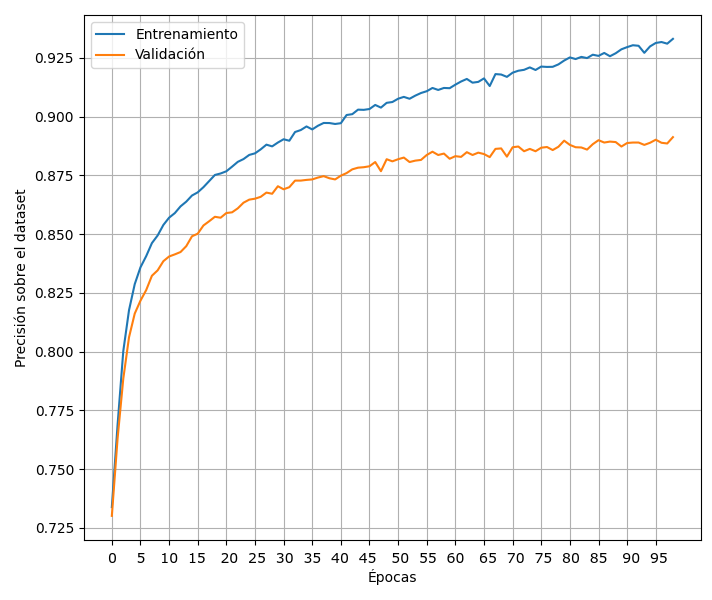
\includegraphics[scale=.22]{figs/exp1/exp1_acc.png}
    \caption{}
    \label{fig:exp1_acc}
  \end{subfigure}
  \hspace{0.05\textwidth}
  \begin{subfigure}[b]{0.45\textwidth}
    \centering
    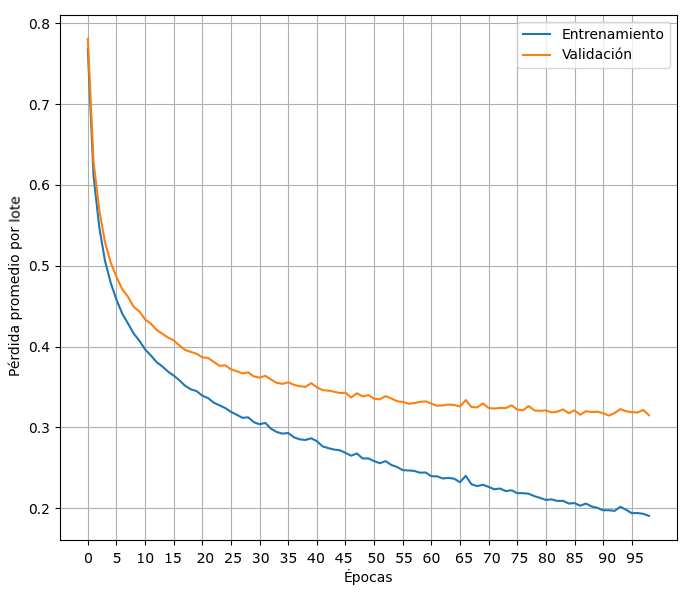
\includegraphics[scale=.22]{figs/exp1/exp1_loss.png}
    \caption{}
    \label{fig:exp1_loss}
  \end{subfigure}
  % Main caption for both subfigures
  \caption{(a) Exactitud por época del experimento 1, (b) Error promedio por lote por época del experimento 1.}
  \label{fig:exp1}
\end{figure}

Lo que se observa es que el entrenamiento se hizo durante las 100 épocas preestablecidas, o sea que el criterio de detención temprana nunca se activó, lo cual quiere decir que la convergencia es monótona pero lenta. Se puede ver que todo el proceso fue bastante regular, en el sentido que las curvas siempre mantuvieron su tendencia (creciente en la exactitud y decreciente en la pérdida) y de una forma ``suave'', sin saltos notorios.

\subsection{Experimento 2}
En este segundo experimento, llevamos a cabo dos modificaciones de hiperparámetros. Por un lado, modificamos el optimizador de SGD a Adam, y por el otro aumentamos el dropout de \(p=0.2\) a \(p=0.3\).

Los resultados obtenidos en este caso se encuentran en los gráficos \ref{fig:exp2_acc} y \ref{fig:exp2_loss}.

\begin{figure}[htbp]  % 'htbp' lets LaTeX choose the best position for the figure
  \centering
  \begin{subfigure}[b]{0.45\textwidth}
    \centering
    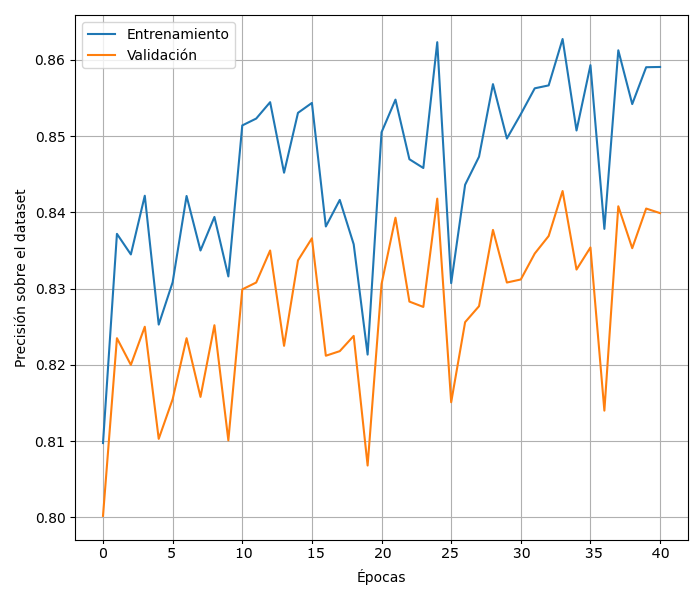
\includegraphics[scale=.22]{figs/exp2/exp2_acc.png}
    \caption{}
    \label{fig:exp2_acc}
  \end{subfigure}
  \hspace{0.05\textwidth}
  \begin{subfigure}[b]{0.45\textwidth}
    \centering
    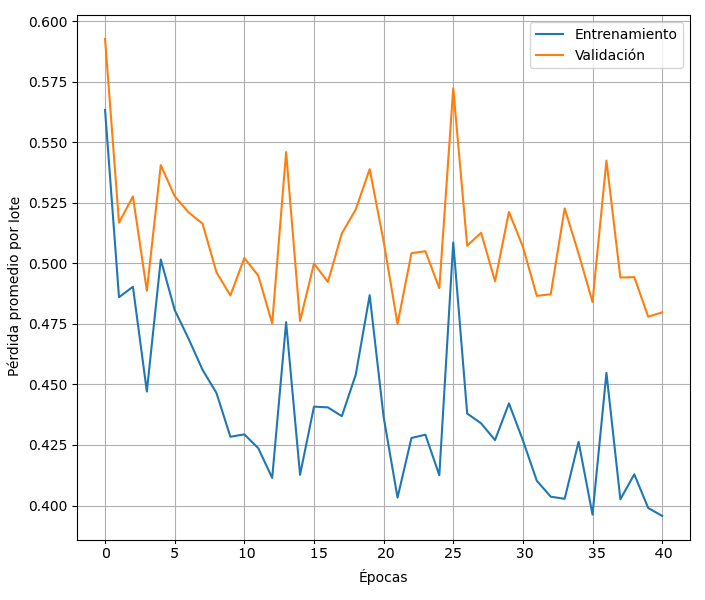
\includegraphics[scale=.22]{figs/exp2/exp2_loss.png}
    \caption{}
    \label{fig:exp2_loss}
  \end{subfigure}
  % Main caption for both subfigures
  \caption{(a) Exactitud por época del experimento 2, (b) Error promedio por lote por época del experimento 2.}
  \label{fig:exp2}
\end{figure}

Lo más notorio de estos gráficos es que si bien se nota una tendencia en ambos (en el de exactitud una tendencia ascendente, y en el de error descendente), esta es muy fluctuante, aumentando y disminuyendo violenta e irregularmente, al contrario del caso anterior. De a momento se alcanzan picos bajos, lo que podría estar indicando un desajuste, y en otras épocas hay picos altos, lo que podría estar indicando un sobreajuste. Dicho todo esto, para intentar corregir estas oscilaciones, en el próximo experimento uno de los cambios que haremos es sobre la tasa de aprendizaje.

\subsection{Experimento 3}
Aquí, a partir de los cambios introducidos en el ensayo anterior, modificamos la tasa de aprendizaje de \(\eta=0.01\) a \(\eta=0.001\) y el tamaño de lote de 100 a 200.

Los gráficos \ref{fig:exp3_acc} y \ref{fig:exp3_loss} reflejan los valores obtenidos a lo largo de las diferentes épocas. 

\begin{figure}[htbp]  % 'htbp' lets LaTeX choose the best position for the figure
  \centering
  \begin{subfigure}[b]{0.45\textwidth}
    \centering
    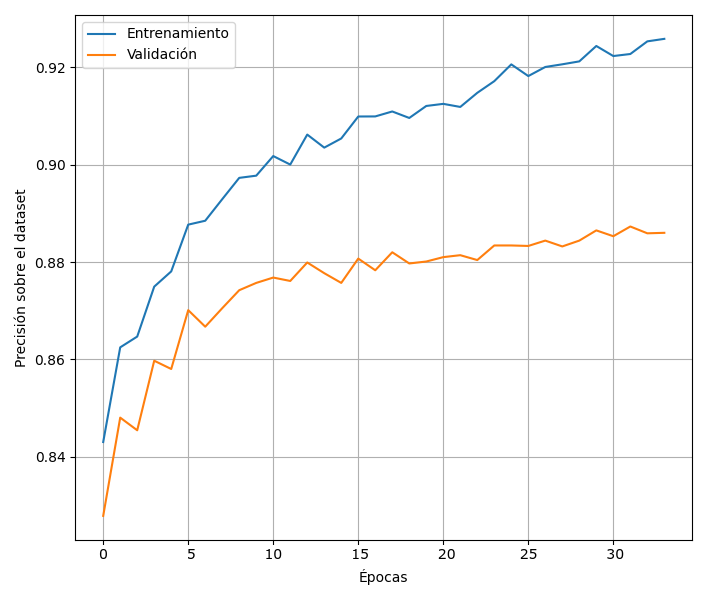
\includegraphics[scale=.22]{figs/exp3/exp3_acc.png}
    \caption{}
    \label{fig:exp3_acc}
  \end{subfigure}
  \hspace{0.05\textwidth}
  \begin{subfigure}[b]{0.45\textwidth}
    \centering
    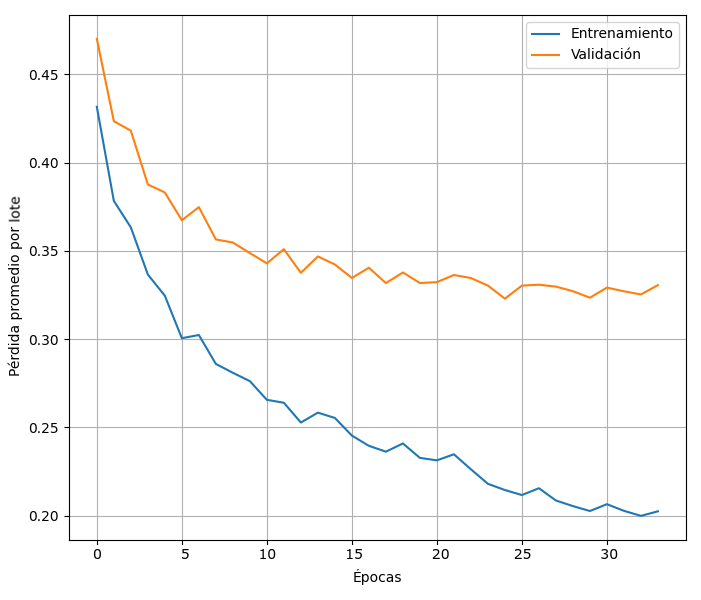
\includegraphics[scale=.22]{figs/exp3/exp3_loss.png}
    \caption{}
    \label{fig:exp3_loss}
  \end{subfigure}
  % Main caption for both subfigures
  \caption{(a) Exactitud por época del experimento 3, (b) Error promedio por lote por época del experimento 3.}
  \label{fig:exp3}
\end{figure}

Se ve claramente cómo las curvas se suavizaron, adquiriendo un comportamiento parecido al del Experimento 1, y llegando a valores finales muy cercanos, pero con muchas menos épocas gracias a la detención temprana: 35 contra 100.

\subsection{Experimento 4}
Finalmente, el último ajuste que hicimos fue, en adición a los de los experimentos 2 y 3, la reducción a la mitad de las neuronas en cada capa oculta, pasando de \(n_1=128\) a \(n_1=64\) en la primera y de \(n_2=64\) a \(n_2=32\) en la segunda.

El comportamiento de la red en esta prueba puede verse en los gráficos \ref{fig:exp4_acc} y \ref{fig:exp4_loss}.

\begin{figure}[htbp]  % 'htbp' lets LaTeX choose the best position for the figure
  \centering
  \begin{subfigure}[b]{0.45\textwidth}
    \centering
    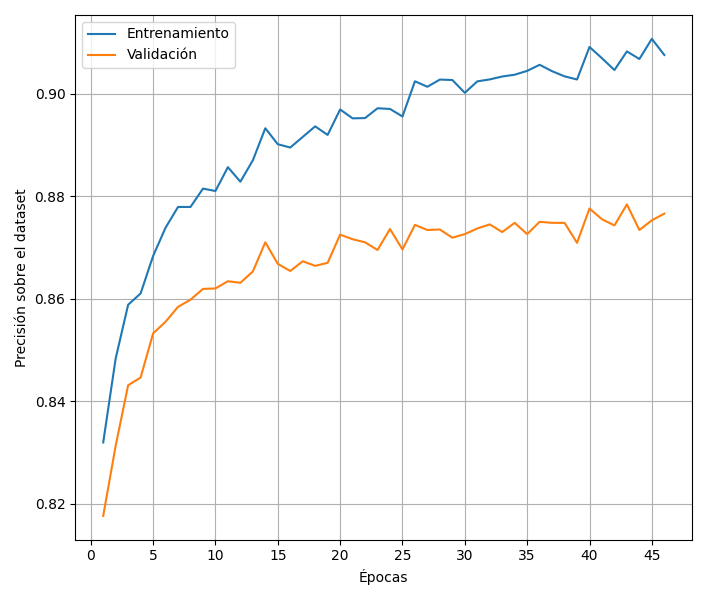
\includegraphics[scale=.22]{figs/exp4/exp4_acc.png}
    \caption{}
    \label{fig:exp4_acc}
  \end{subfigure}
  \hspace{0.05\textwidth}
  \begin{subfigure}[b]{0.45\textwidth}
    \centering
    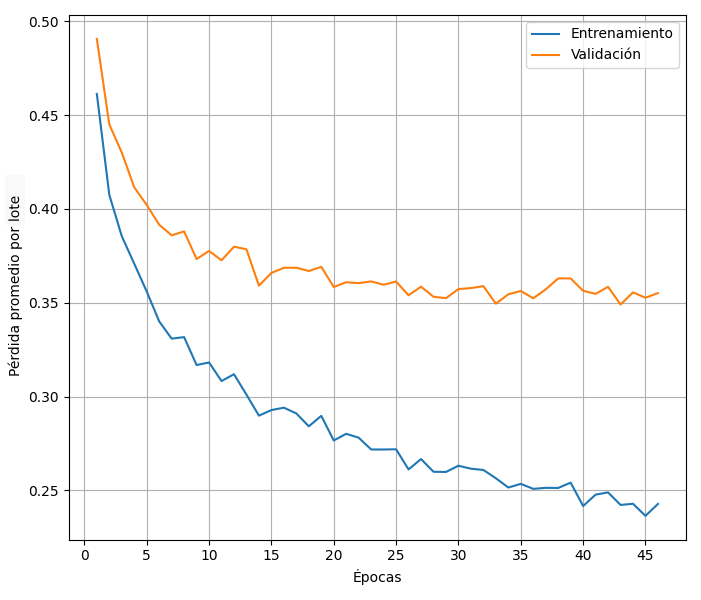
\includegraphics[scale=.22]{figs/exp4/exp4_loss.png}
    \caption{}
    \label{fig:exp4_loss}
  \end{subfigure}
  % Main caption for both subfigures
  \caption{(a) Exactitud por época del experimento 4, (b) Error promedio por lote por época del experimento 4.}
  \label{fig:exp4}
\end{figure}

Observamos un comportamiento bastante regular y suave, con valores finales cercanos a los de los experimentos 1 y 3. Esto podría estar indicando que inicialmente el modelo contaba con más neuronas de las que realmente necesitaba.

\section{Discusión}
% \vspace{-15pt}
En la tabla \ref{tab:experimentos}, se encuentran resumidos los resultados cuantitativos obtenidos en los diferentes experimentos. La columna a de ``Error'' representa el mejor error promedio por lote en una época, teniendo en cuenta el criterio de detención temprana, y la de ``exactitud'' es la exactitud obtenida en dicha época.

\begin{table}[h!]
\centering
\begin{tabular}{lcc|cc}
\toprule
\multirow{2}{*}{\textbf{Experimento}} \hspace{3pt} & \multicolumn{2}{c|}{\textbf{Entrenamiento}} & \multicolumn{2}{c}{\textbf{Validación}} \\
& \textbf{Exactitud} \hspace{3pt} & \textbf{Error} \hspace{3pt} & \hspace{3pt} \textbf{Exactitud} \hspace{3pt} & \textbf{Error} \\
\midrule
Experimento 1  & 93.38\% & 0.1877 & 89.13\% & 0.3151  \\
Experimento 2  & 86.33\% & 0.3807 & 84.05\% & 0.4677  \\
Experimento 3  & 92.74\% & 0.1929 & 88.83\% & 0.3183  \\
Experimento 4  & 91.01\% & 0.2354 & 87.72\% & 0.3458  \\
\bottomrule
\end{tabular}
\caption{Resultados de los experimentos con métricas de exactitud y error promedio por lote.}
\label{tab:experimentos}
\end{table}

Por cuestiones de espacio, el número de época en el que se obtuvieron los valores de la tabla no fue añadido, pero fueron los siguientes: para el Experimento 1, 100 épocas; para el 2, 42; para el 3, 35; y para el 4, 47.

Como primera conclusión, podemos ver que, si bien en todos los gráficos las curvas se ``separan'', no parece haber habido sobreajuste en ningún caso ya que las diferencias entre la exactitud en el conjunto de entrenamiento y validación no son muy grandes, y para validación se obtuvieron buenos valores (en promedio, 90\% de exactitud).

La red con peor desempeño, por una diferencia significativa, fue la segunda, mientras que en las otras tres se muestran resultados muy buenos y similares. Si bien la primera fue la que obtuvo las mejores métricas, también fue la que más tiempo demoró. Si tuviéramos que elegir un modelo, consideramos que el tercero es el mejor: los valores obtenidos son elevados y es el que menos épocas requirió para alcanzarlos.

A partir de los resultados, se puede ver que pequeñas variaciones en los hiperparámetros o en el diseño del modelo pueden tener un impacto significativo en el tiempo de convergencia o en la estabilidad del entrenamiento. Esto pone de manifiesto la importancia de experimentar con diferentes configuraciones y de aplicar técnicas como la detención temprana para evitar entrenamientos innecesariamente largos o con resultados subóptimos.

\section{Conclusiones}
El presente trabajo dio una introducción a los conceptos teóricos fundamentales de las Redes Neuronales, con el objetivo de lograr entender su comportamiento desde lo más básico. También se estudió cómo se lleva a cabo el entrenamiento de una red, y algunos de los hiperparámetros que pueden influir en su desempeño. Para visualizar esto, se diseñó una red para resolver un problema de clasificación de imágenes y, para su entrenamiento, se fue experimentando con diferentes ajustes observando los resultados obtenidos en cada caso, reflejando de esta forma la importancia de comprender el significado de cada uno. De esta forma, se logró no solo construir un modelo funcional, sino también entender mejor los principios que subyacen en el proceso de entrenamiento y su aplicación práctica.

\section{Agradecimientos}
Agradecemos a FAMAF y a la cátedra por motivarnos, y darnos el espacio y las herramientas para llevar a cabo este proyecto. 

% \bibliographystyle{apsrev4-2}
\bibliographystyle{apalike}
\bibliography{refs}

% If in two-column mode, this environment will change to single-column
% format so that long equations can be displayed. Use
% sparingly.
%\begin{widetext}
% put long equation here
%\end{widetext}

% figures should be put into the text as floats.
% Use the graphics or graphicx packages (distributed with LaTeX2e)
% and the \includegraphics macro defined in those packages.
% See the LaTeX Graphics Companion by Michel Goosens, Sebastian Rahtz,
% and Frank Mittelbach for instance.
%
% Here is an example of the general form of a figure:
% Fill in the caption in the braces of the \caption{} command. Put the label
% that you will use with \ref{} command in the braces of the \label{} command.
% Use the figure* environment if the figure should span across the
% entire page. There is no need to do explicit centering.

% \begin{figure}
% \includegraphics{}%
% \caption{\label{}}
% \end{figure}

% Surround figure environment with turnpage environment for landscape
% figure
% \begin{turnpage}
% \begin{figure}
% \includegraphics{}%
% \caption{\label{}}
% \end{figure}
% \end{turnpage}

% tables should appear as floats within the text
%
% Here is an example of the general form of a table:
% Fill in the caption in the braces of the \caption{} command. Put the label
% that you will use with \ref{} command in the braces of the \label{} command.
% Insert the column specifiers (l, r, c, d, etc.) in the empty braces of the
% \begin{tabular}{} command.
% The ruledtabular enviroment adds doubled rules to table and sets a
% reasonable default table settings.
% Use the table* environment to get a full-width table in two-column
% Add \usepackage{longtable} and the longtable (or longtable*}
% environment for nicely formatted long tables. Or use the the [H]
% placement option to break a long table (with less control than 
% in longtable).
% \begin{table}%[H] add [H] placement to break table across pages
% \caption{\label{}}
% \begin{ruledtabular}
% \begin{tabular}{}
% Lines of table here ending with \\
% \end{tabular}
% \end{ruledtabular}
% \end{table}

% Surround table environment with turnpage environment for landscape
% table
% \begin{turnpage}
% \begin{table}
% \caption{\label{}}
% \begin{ruledtabular}
% \begin{tabular}{}
% \end{tabular}
% \end{ruledtabular}
% \end{table}
% \end{turnpage}

%\section{Aknowledgments}


% Specify following sections are appendices. Use \appendix* if there
% only one appendix.
\end{document}
%
% ****** End of file apstemplate.tex ******


